% ****** Start of file apssamp.tex ******
%
%   This file is part of the APS files in the REVTeX 4.1 distribution.
%   Version 4.1r of REVTeX, August 2010
%
%   Copyright (c) 2009, 2010 The American Physical Society.
%
%   See the REVTeX 4 README file for restrictions and more information.
%
% TeX'ing this file requires that you have AMS-LaTeX 2.0 installed
% as well as the rest of the prerequisites for REVTeX 4.1
%
% See the REVTeX 4 README file
% It also requires running BibTeX. The commands are as follows:
%
%  1)  latex apssamp.tex
%  2)  bibtex apssamp
%  3)  latex apssamp.tex
%  4)  latex apssamp.tex
%
\documentclass[%
 reprint,
nofootinbib,
%superscriptaddress,
%groupedaddress,
%unsortedaddress,
%runinaddress,
%frontmatterverbose,
%preprint,
%showpacs,preprintnumbers,
%nofootinbib,
%nobibnotes,
%bibnotes,
 amsmath,amssymb,
 aps,
%pra,
%prb,
%rmp,
%prstab,
%prstper,
%floatfix,
]{revtex4-1}

\usepackage[utf8]{inputenc}
\usepackage[english]{babel}
\usepackage{dsfont}
\usepackage{graphicx}% Include figure files
\usepackage{dcolumn}% Align table columns on decimal point
\usepackage{bm}% bold math
\usepackage{amsmath}
\usepackage{varioref}
\usepackage[bottom]{footmisc}

\usepackage{algpseudocode}
\usepackage{listings}

\newcommand{\RN}[1]{%
  \textup{\uppercase\expandafter{\romannumeral#1}}%
}

%\usepackage{hyperref}% add hypertext capabilities
%\usepackage[mathlines]{lineno}% Enable numbering of text and display math
%\linenumbers\relax % Commence numbering lines

%\usepackage[showframe,%Uncomment any one of the following lines to test
%%scale=0.7, marginratio={1:1, 2:3}, ignoreall,% default settings
%%text={7in,10in},centering,
%%margin=1.5in,
%%total={6.5in,8.75in}, top=1.2in, left=0.9in, includefoot,
%%height=10in,a5paper,hmargin={3cm,0.8in},
%]{geometry}

\begin{document}

%\preprint{APS/123-QED}

\title{Solving the 1D Poisson equation}% Force line breaks with \\

\author{Ivar Svalheim Haugerud}\homepage{http://www.github.uio.no/ivarsh/FYS4150}
\author{Cecilie Glittum}\homepage{http://www.github.uio.no/cecilgl/FYS4150}

\affiliation{%
 Department of Physics, University of Oslo\\
}%


\date{\today}% It is always \today, today,
             %  but any date may be explicitly specified

\begin{abstract}
We solve numerically the one dimensional Poisson equation with Dirichlet boundary conditions. The equation is discretized which makes us able to write the problem as a set of linear equations, and then solve the equation by Gaussian elimination. As the matrix we're studying is tridiagonal, we develop an efficient algorithm for solving the system. We end up with two algorithms, one for a general tridiagonal matrix, which uses $8n$ FLOPS, and one for our special case, which uses $4n$ FLOPS. We find that if we were to use the standard LU decomposition algorithm, it would use $3n^3/2$ FLOPS, and store too much data for our memory when $n$ gets large. When solving problems numerically it is important to spesialize the algorithm for the problem you want to solve. This can reduce computation time while giving the exact same result as a more general algorithm. It is important to use the optimal steplength, we found that we minimize the error by chosing a steplength equal to $10^{-5.5}$.
\end{abstract}


\maketitle


\section{Introduction}

Linear second order differential equations (DEs) on the form
\begin{equation}\label{eq: 2nd order DE}
\frac{d^2 u}{dx^2} + q(x) u(x) = f(x)
\end{equation}
are important in several contexts in physics. In electromagnetism we have Poisson's equation, which is an DE for the electrostatic potential $\Phi$ generated by a localized charge distribution $\rho(\vec{r})$. The equation reads
\begin{equation}
\nabla^2\Phi = -4\pi\rho(\vec{r}).
\end{equation}
By considering a spherical symmetric charge distribution and potential, Poisson's equation simplifies to
\begin{equation}
\frac{1}{r^2}\frac{d}{dr}\left( r^2 \frac{d\Phi}{dr} \right) = -4\pi\phi(r),
\end{equation}
which can be rewritten to
\begin{equation}
\frac{d^2\phi}{dr^2} = -4\pi r \rho(r)
\end{equation}
by the substitution $\Phi(r) = \phi(r)/r$.
This is a linear second order DE of the form given in Eq. \eqref{eq: 2nd order DE} with $\phi \rightarrow u$, $r \rightarrow x$ and $f(x) = 4\pi x \rho(x)$. The equation then reads
\begin{equation}
-\frac{d^2 u}{dx^2} = f(x).
\end{equation}
We want to solve this equation with Dirichlet boundary conditions, in this case $u(0) = u(1) = 0$, for $x \in [0,1]$.

Here, we use three different algorithms to solve the one dimensional Poisson equation. The first algorithm is based on Gaussian elimination, but considers a more general case. The second algorithm is a specialization of the general algorithm, while the third algorithm uses LU decomposition.


\section{Algorithms}

The problem we want to solve, has an analytical solution, but we want to solve it numerically.
To solve the problem numerically we need to discretize the equation. Instead of having continuous functions we get
\begin{align}
  \begin{split}
  x    \rightarrow x_i &\in [x_0, x_1, x_2, \hdots, x_i, \hdots, x_{n+1}]  \\
  u(x) \rightarrow u(x_i) = u_i &\in [u_0, u_1, u_2, \hdots, u_i, \hdots, u_{n+1}]\\
  f(x) \rightarrow f(x_i) = f_i &\in [f_0, f_1, f_2, \hdots, f_i, \hdots, f_{n+1}].
  \end{split}
\end{align}
The value for $x$ is given by $x_i = x_0 + ih$, where $h$ is defined as $h=(x_{n+1}-x_0)/(n+1)$. For our system we let $x$ go from $0$ to $1$, which means that $h$ is given by $h=1/(n+1)$.\\
To solve Poisson's equation numerically, we need an discrete approximation to the double derivative. An expression for this can be found by Taylor expansion of $u(x \pm h)$ around $x$.
\begin{equation}
  u(x\pm h) = u(x) \pm h u^{\prime}(x) + \frac{h^2 u^{\prime\prime}(x)}{2!} \pm  \frac{h^3 u^{\prime\prime\prime}(x)}{3!} + \mathcal{O}(h^4).
\end{equation}
Poisson's equation contains only the double derivative of $u(x)$. We see that we cancel the first and third derivatives by calculating
\begin{equation}
 u(x+h)+u(x-h) = 2u(x) + \frac{2h^2u^{\prime\prime}}{2!} + \mathcal{O}(h^4).
\end{equation}
This equation can be solved for $u^{\prime\prime}$, which gives us
\begin{equation}
  u^{\prime\prime}(x) = \frac{u(h+h)+u(x-h)-2u(x)}{h^2} + \mathcal{O}(h^2) \label{u_double_d_continous}.
\end{equation}
In our Taylor expansion, the truncation error was proportional to $h^4$, but since we divide by $h^2$ in the approximation of the double derivative, the truncation error in this approximation is proportional to $h^2$.
Since we are not working with continuous functions we discretize the function by writing  $f_{i}$ instead of $f(x)$ and $u_{i\pm 1}$ instead of $u(x\pm h)$. With this notation Eq. \eqref{u_double_d_continous} becomes
\begin{equation}
  f_i = -\frac{u_{i+1} + u_{i-1} - 2{u_i}}{h^2} + \mathcal{O}(h^2). \label{all_gore}
\end{equation}
When we calculate this numerically we will not include the end points of our system, since these are set by our boundary conditions, $u_0=u_{n+1}=0$. To get a better understanding of this algorithm we will write out the terms, and define a new array $\vec{f^{*}} = h^2\vec{f}$ to make it simpler
\begin{align*}
  f^{*}_1 &= -u_2 - u_0 + 2u_1 \\
  f^{*}_2 &= -u_3 - u_1 + 2u_2 \\
  f^{*}_3 &= - u_4 - u_2 + 2u_3. \\
         \vdots& \\
  f^{*}_{n} &= -u_{n+1} - u_{n-1} + 2u_{n}
\end{align*}
  If we have any history working with linear algebra we can see that this set of equations can be translated to a linear algebra problem. Eq. \eqref{all_gore} can be written as a matrix-vector product
\begin{equation}
  \hat{A} \vec{u} = \vec{f}^{*}, \label{system}
\end{equation}
where $f\in\mathds{R}^{n}$ and $\hat{A}$ is an $n\times n$ matrix defined as
\begin{equation}
  \hat{A} = \begin{bmatrix}
               2& -1 & 0 & \dots & 0 \\
               -1 & 2 & -1 &\dots &\vdots \\
               0 & -1 & 2 & \dots  & \vdots \\
               \vdots & \vdots & \vdots & \ddots &\vdots\\
               0 &  \vdots   & \vdots  & \dots & 2 \\
            \end{bmatrix}
\end{equation}
For our problem we know what $\vec{f}^*$ is, and we want to solve for $\vec{u}$. $f(x)$ is defined as
\begin{equation}
  f(x) = 100e^{-10x},
\end{equation}
which we will need to use in our numerical solution. Using the method described above we will be able to approximate $u$ very accurately. Since the system has an analytical solution,
\begin{equation}
  u(x) = 1-(1-e^{-10})x-e^{-10x}, \label{analytic_solv}
\end{equation}
we can test our numerical results against the analytical. To do this we will use the following expression for the relative error
\begin{equation}
  \epsilon = \log_{10} \left( \frac{ \lvert u_{\mathrm{num}} -u_{\mathrm{ana}}\rvert }{ \lvert  u_{\mathrm{num}} \rvert } \right) \label{calc_deviation}
\end{equation}
We will not include the endpoints ($i = 0$ and $i =  n+1$) in any of our algorithms, since these are fixed to a value of zero. Therefore our indexing will start at $1$ and end at $n$, while the values for index $0$ and $n+1$ are set to zero. \par

\subsection{Gaussian elimination of tridiagonal matrix}
Eq. \eqref{system} would solve the 1D Poisson equation, but in the beginning we want to be a bit more general. Our matrix is tridiagonal, so we solve the problem for a general tridiagonal matrix where none of the elements are necessary equal.

For the computation algorithm to be as fast as possible we will not define an $n\times n$ array. This would lead to storing $n^2$ double elements in our computer, and we would run out of memory fast. Since most of our matrix is zero's, we will instead only use the three vectors along the diagonal, and find the the algorithm by just using these vectors.

We will therefore make our matrix $\hat{A}$ consist of three different vectors, $a,c\in \mathds{R}^{n-1}$, and $b\in \mathds{R}^{n}$
\begin{equation}
  \hat{A} =
\begin{bmatrix}
       b_1& c_1 & 0 &\dots   & \dots &\dots \\
       a_1 & b_2 & c_2 &\dots &\dots &\dots \\
       & a_2 & b_3 & c_3 & \dots & \dots \\
       & \dots   & \dots &\dots   &\dots & \dots \\
       &   &  &a_{n-2}  &b_{n-1}& c_{n-1} \\
       &    &  &   &a_{n-1} & b_n \\
\end{bmatrix}
\end{equation}
The general algorithm for solving $\hat{A}\vec{u} = \vec{f}^*$ needs only two steps, a forward substitution and a backward substitution. We will derive this formula by using Gaussian elimination on the equation. \\

Let's find the general algorithm by using a $4\times4$ matrix and look for a pattern. Our system can then be written as
\begin{align*}
  \hat{A} \vec{u} &= \vec{f}^{*} \\
  \begin{bmatrix}
      b_1 & c_1 & 0   & 0   \\
      a_1 & b_2 & c_2 & 0   \\
      0   & a_2 & b_3 & c_3 \\
      0   & 0   & a_3 & b_4
  \end{bmatrix}
  \begin{bmatrix} u_1 \\ u_2 \\ u_3 \\ u_4 \end{bmatrix}
    &=
  \begin{bmatrix} f^{*}_1 \\ f^{*}_2 \\ f^{*}_3 \\ f^{*}_4 \end{bmatrix}
\end{align*}
The system we will use Gaussian elimination on, to transform the first $4\times 4$ elements into the identity operator, is therefore
\begin{equation}
  \begin{bmatrix}
      b_1 & c_1 & 0   & 0 &   f^{*}_1  \\
      a_1 & b_2 & c_2 & 0 &   f^{*}_2  \\
      0   & a_2 & b_3 & c_3 & f^{*}_3 \\
      0   & 0   & a_3 & b_4 & f^{*}_4
  \end{bmatrix} \label{gaussian_elimination}
\end{equation}
First we use the forward substitution to remove all of the elements along the bottom diagonal. To remove element $a_i$ we multiply the line above $a_i$ (line $i$) by a constant $a_i/b_i$ which will make the element which was previously equal to $b_i$ equal to $a_i$. After this is done we subtract row $i$ from row $i+1$, and the element which originally was $a_i$ will then be equal to zero. This easier to see by doing the calculations. We multiply row $\RN{1}$ of \eqref{gaussian_elimination} by $a_1/b_1$ to fulfil the requirement just stated, and subtract this from row $\RN{2}$ to get
\begin{equation}
  \begin{bmatrix}
      b_1 & c_1   & 0   & 0 &   f^{*}_1             \\
      0 & b_2-c_1a_1/b_1 & c_2 & 0 &   f^{*}_2- f^{*}_1a_1/b_1  \\
      0   & a_2 & b_3 & c_3 & f^{*}_3 \\
      0   & 0   & a_3 & b_4 & f^{*}_4
  \end{bmatrix} \label{gaussian_elimination2}
\end{equation}
Since we have started to have some ugly terms in our system we will introduce some new variables to make the algorithm more clear, we therefore define that $\tilde{b}_2 = b_2-c_1a_1/b_1$, and  $\tilde{f}_2 = f^{*}_2- f^{*}_1a_1/b_1$. This definition makes us able to write Eq. \eqref{gaussian_elimination2} as
\begin{equation}
  \begin{bmatrix}
      b_1 & c_1   & 0   & 0 &   f^{*}_1             \\
      0 & \tilde{b}_2 & c_2 & 0 &   \tilde{f}_2  \\
      0   & a_2 & b_3 & c_3 & f^{*}_3 \\
      0   & 0   & a_3 & b_4 & f^{*}_4
  \end{bmatrix} \label{gaussian_elimination3}
\end{equation}
We then have to continue with Gaussian elimination by multiplying line $\RN{2}$ by $a_2/\tilde{b}_2$ and subtracting it from line $\RN{3}$ we get
\begin{equation}
  \begin{bmatrix}
      b_1 & c_1   & 0   & 0 &   f^{*}_1             \\
      0 & \tilde{b}_2 & c_2 & 0 &   \tilde{f}_2  \\
      0   & 0 & b_3-c_2a_2/\tilde{b}_3 & c_3 & f^{*}_3-\tilde{f}_2a_2/\tilde{b}_2 \\
      0   & 0   & a_3 & b_4 & f^{*}_4
  \end{bmatrix} \label{gaussian_elimination4}
\end{equation}
By again using a similar redefinition, $\tilde{b}_3 = b_3-c_2a_2/\tilde{b}_3$ and $\tilde{f}_3 = f^{*}_3-\tilde{f}_2a_2/\tilde{b}_2$, brings us to \eqref{gaussian_elimination4} to
\begin{equation}
  \begin{bmatrix}
      b_1 & c_1   & 0   & 0 &   f^{*}_1               \\
      0 & \tilde{b}_2 & c_2 & 0 &   \tilde{f}_2  \\
      0   & 0 & \tilde{b}_3 & c_3 & \tilde{f}_3\\
      0   & 0   & a_3 & b_4 & f^{*}_4
  \end{bmatrix} \label{gaussian_elimination10}
\end{equation}
From these calculations we can see the pattern. Doing the forward substitution gives us the expression for a general $\tilde{b}_i$ and $\tilde{f}_i$
\begin{align}
  \tilde{b}_i &= b_i - \frac{c_{i-1}a_{i-1}}{\tilde{b}_{i-1}}, \label{eq: btilde} \\
  \tilde{f}_i &= f^{*}_i - \frac{\tilde{f}_{i-1}a_{i-1}}{\tilde{b}_{i-1}}. \label{eq: ftilde}
\end{align}
We have now found an algorithm which removes the bottom diagonal array from our matrix. We will now need to do the backward substitution to remove the upper diagonal array in our matrix. From the forward substitution we see that row $\RN{1}$ did not change, but to make the backward substitution algorithm more elegant we define $ \tilde{f}^*_1=f^{*}_1$ and $\tilde{b}_1 = b_1$. The system of equations has become
\begin{equation}
  \begin{bmatrix}
      \tilde{b}_1 & c_1   & 0   & 0 &   \tilde{f}_1             \\
      0 & \tilde{b}_2 & c_2 & 0 &   \tilde{f}_2  \\
      0   & 0 & \tilde{b}_3 & c_3 & \tilde{f}_3\\
      0   & 0   & 0 & \tilde{b}_4 & \tilde{f}_4
  \end{bmatrix} \label{gaussian_elimination5}
\end{equation}
To solve the set of equations, we want the identity matrix for the first $n\times n$ elements. This is easy to achieve for the last row; we simply divide the hole row by $\tilde{b}_4$. The expression we now find in the right most column is the answer we are looking for, we will call this element $u_4 = \tilde{f}_4/\tilde{b}_4$. Our system of equations now looks like
\begin{equation}
  \begin{bmatrix}
     \tilde{b}_1 & c_1   & 0   & 0 &   f^{*}_1               \\
      0 & \tilde{b}_2 & c_2 & 0 &   \tilde{f}_2  \\
      0   & 0 & \tilde{b}_3 & c_3 & \tilde{f}_3\\
      0   & 0   & 0 & 1 & u_4
  \end{bmatrix} \label{gaussian_elimination11}
\end{equation}
To remove $c_3$ we multiply line $\RN{4}$ by $c_3$ and subtract it from line $\RN{3}$. We then find

\begin{equation}
  \begin{bmatrix}
    \tilde{b}_1 & c_1   & 0   & 0 &   f^{*}_1              \\
      0 & \tilde{b}_2 & c_2 & 0 &   \tilde{f}_2  \\
      0   & 0 & \tilde{b}_3 & 0 & \tilde{f}_3-u_4c_3\\
      0   & 0   & 0 & 1 & u_4
  \end{bmatrix} \label{gaussian_elimination12}
\end{equation}
We normalize line $\RN{3}$ by dividing by $\tilde{b}_3$, we then define $u_3 = (\tilde{f}_3-u_4c_3)/\tilde{b}_3$, which gives us
\begin{equation}
  \begin{bmatrix}
      \tilde{b}_1 & c_1   & 0   & 0 &   f^{*}_1              \\
      0 & \tilde{b}_2 & c_2 & 0 &   \tilde{f}_2  \\
      0   & 0 & 1 & 0 & u_3\\
      0   & 0   & 0 & 1 & u_4
  \end{bmatrix} \label{gaussian_elimination13}
\end{equation}
We continue to do this for every row. It is important for this part of the algorithm to start at the bottom, and to work upwards from $i = n-1$ to $i = 1$. Next step would now be to multiply row $\RN{3}$ with $c_2$ and subtract it from row $\RN{2}$, then normalizing by dividing by $\tilde{b}_2$. From these steps we can see the general algorithm for the backward substitution
\begin{equation}\label{eq: u}
  u_i = \frac{\tilde{f}_i-c_iu_{i+1}}{\tilde{b}_i},
\end{equation}
for $i = n-1 , n-2, ..., 1$.
\par
Assuming pre initialized vectors \texttt{a, b, c, f} and defining as shown, $\tilde{f}_1 = f_1$ and $\tilde{b}_1 = b_1$, our general algorithm reads in pseudo code
\begin{algorithmic}[H]
\State
\For {i = 2, 3, ..., n}
	\State quotient $= a_{i-1}/\tilde{b}_{i-1}$;
	\State $\tilde{b}_i = b_i - c_{i-1}*$ quotient;
	\State $\tilde{f}_i = f^*_i - \tilde{f}_{i-1}*$ quotient;
\EndFor
\State
\State compute $u_{n} = \tilde{f}_n/\tilde{b}_n$;
\State
\For {i = n-1, n-2, ..., 1}
	\State $u_i = (\tilde{f}_i - c_i*u_{i+1})/\tilde{b}_i$;
\EndFor
\State
\end{algorithmic}
We are also interested in finding the number of floating point operations (FLOPS) in our algorithm. We see that in the first loop, we do 5 FLOPS for every $i$ and in the second loop we do 3 FLOPS per $i$. Each loop is run $n-1$ times, thus this algorithm has $(8(n-1) + 1) \mathrm{FLOPS} = (8n - 7) \mathrm{FLOPS}$. For large $n$, we can ignore the constant term. Our algorithm therefore uses $8n$ FLOPS. The reason for calculating the quantity \texttt{quotient} is thus to reduce the number of FLOPS from $9n$ to $8n$ as this quantity is used twice in the first loop.

\subsection{Specialized algorithm}

By using the fact that our matrix is a symmetric Toeplitz matrix with the number $2$ along the main diagonal and the number $-1$ along the two other diagonals, we're able to modify our general algorithm with the purpose of making it more efficient for our special case.

When using the general algorithm, we have in the special case $a_i = c_i = -1$ and $b_i = 2$ for all $i$. When inserting these values into the Eqs.\eqref{eq: btilde}, \eqref{eq: ftilde} and \eqref{eq: u} we get
\begin{align}
  \tilde{b}_i &= 2 - \frac{1}{\tilde{b}_{i-1}}, \label{eq: btilde_special} \\
  \tilde{f}_i &= f^{*}_i + \frac{\tilde{f}_{i-1}}{\tilde{b}_{i-1}}, \label{eq: ftilde_special} \\
  u_i &= \frac{\tilde{f}_i + u_{i+1}}{\tilde{b}_i}. \label{eq: u_special}
\end{align}
In appendix \ref{appendix_1}, we show that the recurrence relation for $\tilde{b}_i$, Eq. \eqref{eq: btilde_special} has a solution
\begin{equation}
\tilde{b}_i \equiv \tilde{d}_i = \frac{i+1}{i},
\end{equation}
where we rename the diagonal elements from $b_i$ to $d_i$ to distinguish this result from the general case. This is a general result for our special matrix, and can thus be calculated outside of the algorithm for solving Eq. \eqref{system}. The resulting operations to be done in the algorithm (the parts dependent on the right hand-side of the system) are
 \begin{align}
  \tilde{f}_i &= f^{*}_i + \frac{\tilde{f}_{i-1}}{\tilde{d}_{i-1}}, \label{eq: ftilde_special} \\
  u_i &= \frac{\tilde{f}_i + u_{i+1}}{\tilde{d}_i}. \label{eq: u_special}
\end{align}

The specialized algorithm thus reads
\begin{algorithmic}[H]
\State
\For {i = 2, 3, ..., n}
	\State $\tilde{f}_i = f^*_i + \tilde{f}_{i-1}/\tilde{d}_{i-1}$;
\EndFor
\State
\State compute $u_{n} = \tilde{f}_n/\tilde{b}_n$;
\State
\For {i = n-1, n-2, ..., 1}
	\State $u_i = (\tilde{f}_i + u_{i+1})/\tilde{d}_i$;
\EndFor
\State
\end{algorithmic}

Both the loops now use $2$ FLOPS each time they are run, and each loop runs $n-1$ times. Thus this specialized algorithm uses $(4(n-1) + 1) \mathrm{FLOPS} = (4n - 3) \mathrm{FLOPS}$. For large $n$, the algorithms thus uses $4n$ FLOPS.
As we see, by using the special case for our matrix, we have reduced the algorithm from $8n$ FLOPS to $4n$ FLOPS.

\subsection{LU decomposition}

LU decomposition is a method where a non-singular matrix $\hat{A}$ is rewritten as a product of a lower triangular matrix $\hat{L}$ and an upper triangular matrix $\hat{U}$
\begin{align*}
  \hat{A} &= \hat{L}\hat{U}, \\
  \begin{bmatrix}
      a_{11} & a_{12} & a_{13}  & a_{14}   \\
      a_{21} & a_{22} & a_{23} & a_{24}   \\
      a_{31} & a_{32} & a_{33} & a_{34} \\
      a_{41} & a_{42} & a_{43} & a_{44}
  \end{bmatrix}
  &=
    \begin{bmatrix}
      1 & 0 & 0   & 0   \\
      l_{21} & 1 & 0 & 0   \\
      l_{31} & l_{32} & 1 & 0 \\
      l_{41} & l_{42} & l_{43} & 1
  \end{bmatrix}
    \begin{bmatrix}
      \tilde{u}_{11} & \tilde{u}_{12} & \tilde{u}_{13}  & \tilde{u}_{14}   \\
      0 & \tilde{u}_{22} & \tilde{u}_{23} & \tilde{u}_{24}   \\
      0   & 0 & \tilde{u}_{33} & \tilde{u}_{34} \\
      0   & 0   & 0 & \tilde{u}_{44}
  \end{bmatrix}.
\end{align*}

By writing the matrix $\hat{A}$ as its LU decomposition, we can solve Eq. \eqref{system} in two steps
\begin{equation}
\hat{L}\hat{U}\vec{u} = \vec{f}^* \leftrightarrow \hat{L}\vec{v} = \vec{f}^*, \quad  \hat{U}\vec{u} = \vec{v}.
\end{equation}
As $\hat{L}$ is lower triangular, the equation $\hat{L}\vec{v} = \vec{f}^*$ can be solved by forward substitution, and the remaining equation $\hat{U}\vec{u} = \vec{v}$ can be solved by backward substitution.\\


The approach for numerical simulations is to solve Eq. \eqref{system} with the three different algorithms. We also studied the relative error of the algorithms as function of $n$ by using Eq. \eqref{calc_deviation}. Further we compared the runtimes of the different algorithms.

By reducing the number of FLOPS our code should be able to run faster. By going from $8n$ FLOPS for the general algorithm to $4n$ FLOPS for the specialized algorithm, we expect the code to run twice as fast. This is by assuming that all calculations take the same amount of time. To study this relationship we run both algorithms $1000$ times for different values of $n$ increasing logarithmic linearly. For each value of $n$ we calculate the average and the standard deviation for both algorithms.


\section{Results}
Using our numerical methods we find a graph which matches the analytic solution in Eq. \eqref{analytic_solv}. This is shown in Fig. \vref{analyticalnumerical}, where we have used our special algorithm in particular, even though all methods seems to give the same results.
\begin{figure}
\centering
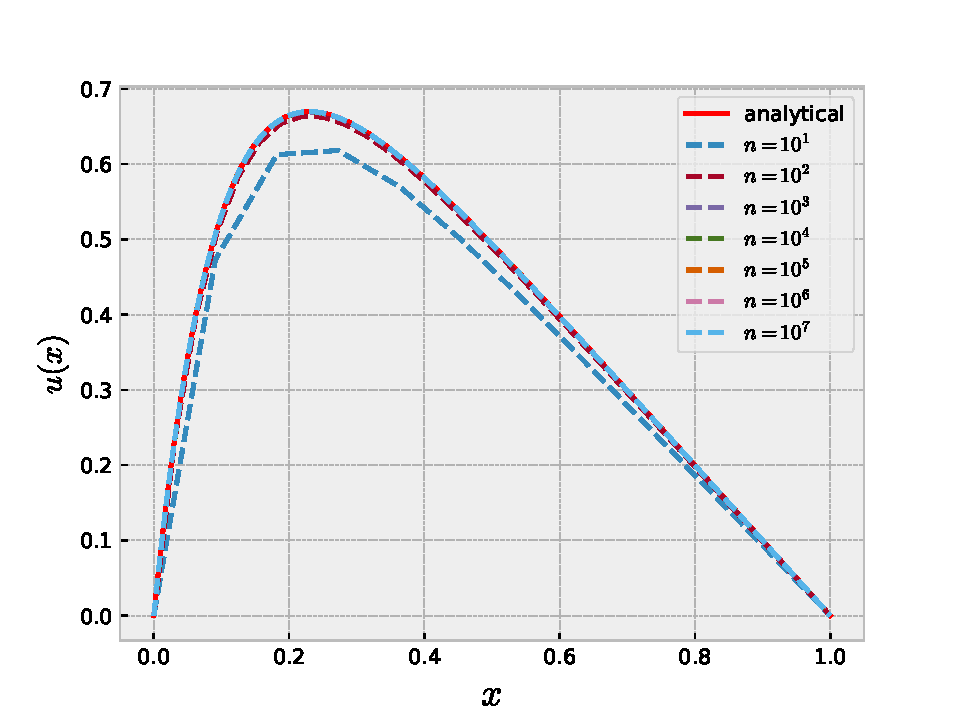
\includegraphics[scale=0.5]{../figures/graphs.pdf}
\caption{The solution of Poisson's equation with boundary conditions $u(0) = u(1) = 0$. The plot shows both the analytical solution as well as the numerical solution found by Gaussian elimination for various values of $n$ using our specialized algorithm.}
\label{analyticalnumerical}
\end{figure}

From this graph it is hard to tell the deviation between the numerical and analytical solution. To get a better understanding of this, we plot the logarithm of the maximum relative deviation in Eq. \eqref{calc_deviation} for each value of $n$. We plot this value versus the logarithm of $n$ to find the maximum error as a function of $n$. This graph is shown in Fig. \ref{error}. In this graph we have used the least squares method to find the best linear fit to the data points. Theory predicts a slope of $-2$, due to the truncation term going as $h^2$. When calculating the slope we find that the slope is $-1.99\pm0.01$, where the uncertainty is calculated from the least squares method \cite{squires}.

We see that the error follows this slope until $\log n  \approx 5.5$. For $n$ bigger than this, the error increases.

\begin{figure}
\centering
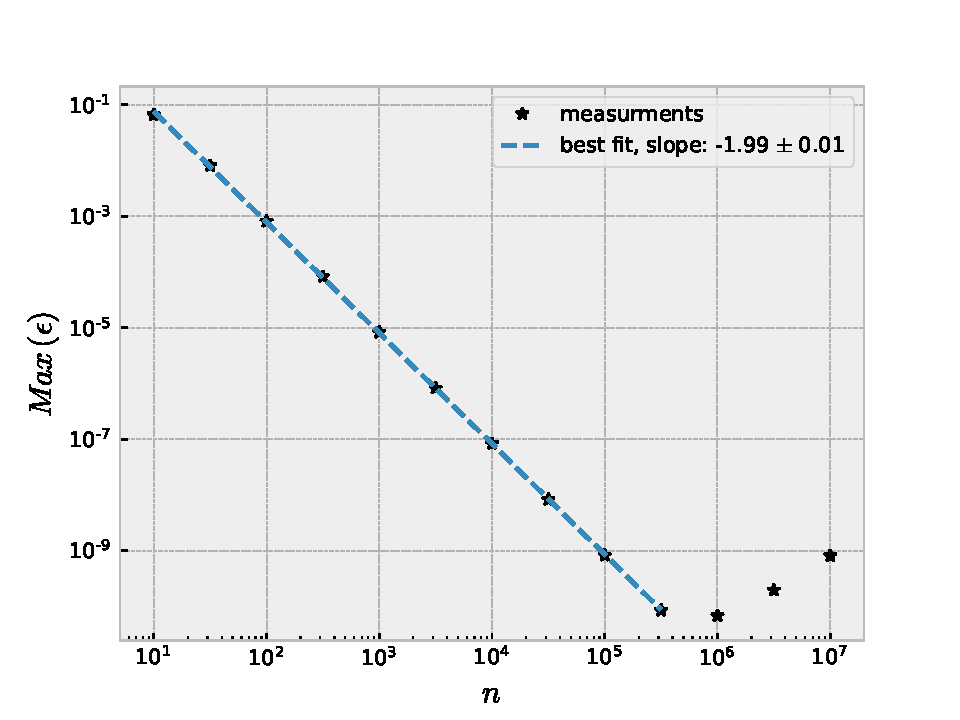
\includegraphics[scale=0.5]{../figures/log_difference.pdf}
\caption{The maximum deviation for each $n$ between the numerical and analytical solution of Poisson's equation. This is shown in a log-log plot to visualize the large differences, and to be able to calculate the slope. By using the least squares method we find that the slope is $-1.99\pm0.01$.}
\label{error}
\end{figure}

\par

To study the relationship between the runtimes of the general and specialized algorithms we ran both algorithms $1000$ times for different values of $n$ increasing logarithmic linearly. How the relationship between two average runtimes depend on $n$ is shown in Fig. \vref{time relationship}. In this graph the relationship is calculated by $\langle t_{8N} \rangle /\langle t_{4N} \rangle$. We see in Fig. \vref{time relationship} that we have a large uncertainty for lower $n$, but as $n$ increases the time relationship stabilizes, and the uncertainty decreases. The value it stabilizes as is calculated to be $2.10\pm0.02$.

\begin{figure}
\centering
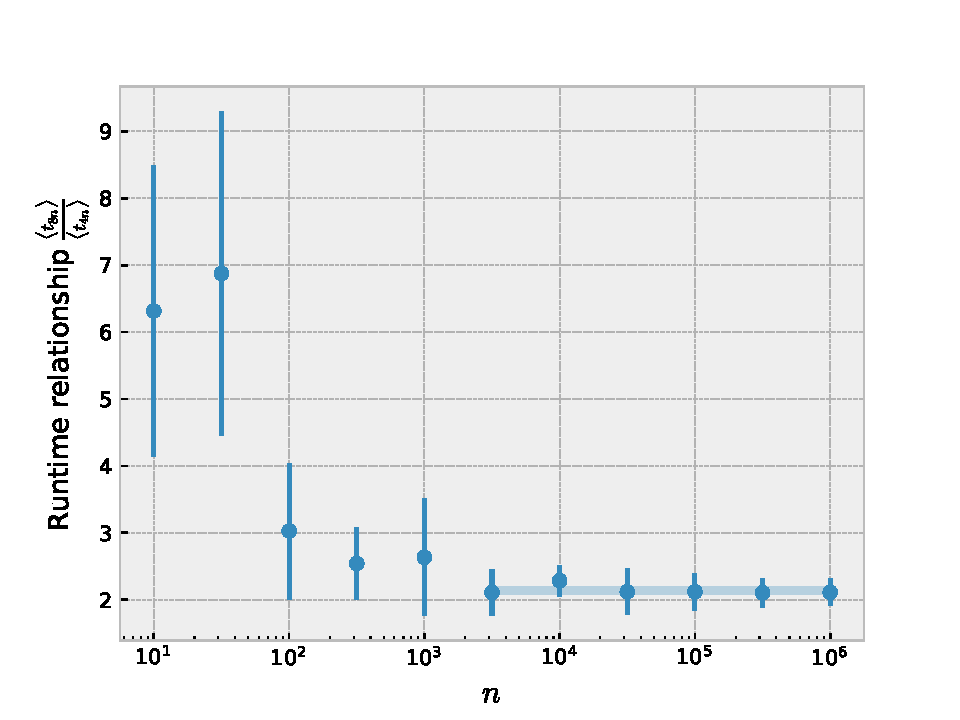
\includegraphics[scale=0.5]{../figures/time_difference.pdf}
\caption{The relationship between the average time for each algorithm calculated by $\langle t_{8n} \rangle /\langle t_{4n} \rangle$. For each $n$ we ran the algorithm $1000$ times and calculated the mean time and standard deviation for these runs. The relationship between the runtimes stabilizes at $2.10\pm0.02$ for $\log n > 3.5$.}
\label{time relationship}
\end{figure}

When we study the time needed for solving the same problem numerically, but using LU decomposition, we find a logarithmic-linearly dependence on $n$. This is shown in Fig. \vref{time relationship_LU}.
We calculate the slope in the log-log-plot to be $2.99\pm0.1$, this corresponds to a runtime proportional to $n^3$ \cite{hjorten}.

\begin{figure}
\centering
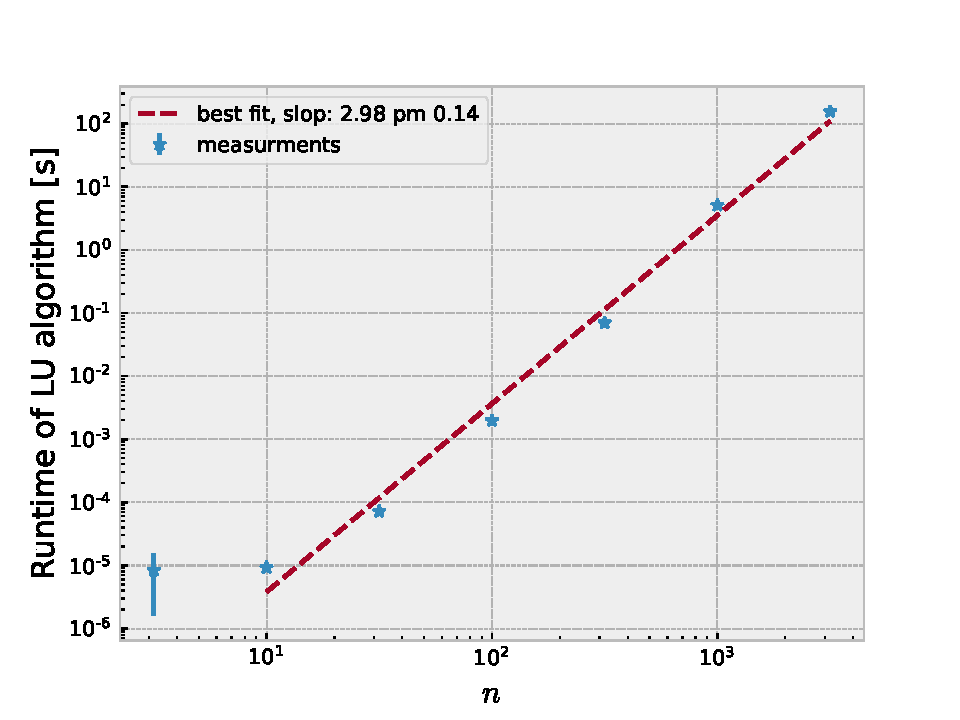
\includegraphics[scale=0.5]{../figures/time_difference_LU.pdf}
\caption{Runtime for LU-decomposition for different values of $n$ for an $n\times n$ matrix. Due to the LU decomposition algorithm being slow we took the average and standard deviation of $7$ runs for each value of $n$.}
\label{time relationship_LU}
\end{figure}

When comparing the results produced by the specialized algorithm and the LU decomposition, we find that the results are exactly the same.

\section{Discussion}
LU is a general algorithm, which works for all non-singular matrices. Our algorithm, using Gaussian elimination, exploits the fact that we are working on a tridiagonal matrix. Instead of storing the whole $n\times n$ matrix we store only the three diagonal arrays. This makes us able to get a highly efficient algorithm compared to the standard LU decomposition which has to work with the whole matrix.\\
As we see in Fig. \vref{time relationship_LU} the time used to calculate the LU decomposition goes as $n$ cubed. This means that for larger values of $n$, the run time becomes intolerable. If we assume that the linear relationship continued we would find that the runtime using the LU decomposition would be around $1.26$ months for $n=10^5$.

By using the Gaussian algorithms the runtimes goes linearly with $n$. The three algorithms gives exactly the same answers, but the specialized algorithm is tailor-made for our problem, which means it will run faster. This means that we can still run the algorithm when $n$ gets large. \\
Another problem by using the LU decomposition algorithm, is that we need to store more information on our computer. If we save $\hat{A}$ as a double $n\times n$ matrix, we need to save $8$ bytes times $n^2$, only to store the data of that single matrix. For example if we want to run the LU decomposition for $n=10^5$, we will need to store $8\times (10^5)^2 = 8 \times 10^{10}$ bytes on our computer. This is $80$ giga bytes. And if we want to store $\hat{L}$ and $\hat{U}$ as well, we need to multiply this by three. To store that much information, when most of the values are zero, is completely unnecessary. LU decomposition would need a lot of memory, and a lot of time, when $n$ gets large. For the general and specialized algorithms, the amount of data we need to store goes linearly with $n$, and makes life easy.
\par
Even though our specialized algorithm gives us the opportunity to run the algorithm for large $n$, we have another restriction on $n$, if we want precise results. When doing differentiation and integration analytically, we let the small change in the function, d$x$, go towards zero. We can not do this numerically due to how computers store numbers. As we can see in Fig. \vref{error} the logarithm of the maximum deviation decreases linearly with the logarithm of $n$. But at $n=10^{5.5}$ this trend stops, and the error gets larger. This error comes from how computers store numbers. Not all numbers can be exactly represented on computers. Since we are storing numbers using $64$ bits in our algorithm, all information about the number, which would need more than those $64$ bits to represent, gets rounded off. This round-off error is very small, but when we do FLOPS, for example subtraction between two very small numbers, the information we lose by round-off can be a large portion of the resulting number. This error will then play an important part in the resulting answer, and might propagate onwards in our calculation. If we increase $n$ further than what we did in Fig. \vref{error} we will see that the deviation gets even larger.
\par
By using the fact that all the elements in each array were $1$'s and $2$'s we were able to optimize our algorithm further, by reducing the number of FLOPS from $8n$ to $4n$. The relationship between the run times for these two algorithms is shown in Fig. \vref{time relationship}. As one would expect, the relationship stabilizes around $2$ when $n$ increases. For lower values of $n$ the relationship has a higher standard deviation, and is quite far away from $2$, so what is going on here?\\
There is more than just the FLOPS that is happening in our algorithm. For every operation the code also needs to read and write data, and index the arrays. \\
All FLOPS are not equivalent in computational time. For example is division more numerically challenging than addition for the computer, and will therefore take longer time. \\
This is the effect we see for low $n$. When there are few total operations there are other effects and operations which are more significant, which dictates the time-relationship between the two algorithms. We should therefore not assume to half the runtime for small $n$. As $n$ increases the number of FLOPS increases, and we see that the relationship stabilizes at around $2$. The other operations don't effect the total runtime as much when the number of FLOPS is large. From the graph we can also tell that the standard deviation of the mean runtime is much larger for small $n$, there is more at play here than meets the eye. For example is the resolution of the clock used at $\mu$ seconds, and for small $n$ the runtime of the code is the same order of magnitude as the resolution of the clock.\\
The fact that the LU decomposition gives the exact same result as our own, spezialized algorithm, indicates that the algorithm, and it's implimentation, is correct.

\section{Conclusion}

We have solved the one dimensional Poisson equation, with Dirichlet boundary conditions, numerically. By discretizing the equation we are able to represent the problem as a set of equations, and solve it using Gaussian elimination. We developed an algorithm for solving this problem for a general tridiagonal matrix. This algorithm had $8n$ FLOPS, and was much more efficient, and used less memory, than a LU algorithm for an $n\times n$ matrix, which made it possible to use large values of $n$.\\
We were able to optimize the algorithm even further by creating an algorithm for the matrix used in our system. This algorithm used $4n$ FLOPS, and resulted in running twice as fast as the $8n$ FLOPS algorithm. \\
Even though LU decomposition can solve the set of equations for any matrix, it uses $3n^3/2$ flops, and requires more memory. It is therefore important to specialize algorithms for the specific problem you want to solve, even though it is less general, to reduce the computation time and memory usage.

\section{Comments}
All of the code used is available on our github \footnote{\url{http://www.github.uio.no/cecilgl/FYS4150}, and \url{http://www.github.uio.no/ivarsh/FYS4150}}. Here the \texttt{README.MD} files will describe the structure of our github, and what each program was used for. The code itself will also include notes explaining what we do.

\appendix

\section{Analytical expression for $\tilde{d}_i$}\label{appendix_1}

$\tilde{d}_i$ is given by the recurrence relation
\begin{equation}\label{eq: difference eq}
\tilde{d}_i = 2 - \frac{1}{\tilde{d}_{i-1}},
\end{equation}
with the initial condition $\tilde{d}_1 = 2$. We can thus calculate the following values for $\tilde{d}_i$:
\begin{align*}
\tilde{d}_2 &= 2 - \frac{1}{\tilde{d}_{1}} = 2 - \frac{1}{2} = \frac{3}{2}\\
\tilde{d}_3 &= 2 - \frac{1}{\tilde{d}_{2}} = 2 - \frac{1}{\frac{3}{2}} = \frac{4}{3}\\
\tilde{d}_4 &= 2 - \frac{1}{\tilde{d}_{3}} = 2 - \frac{1}{\frac{4}{3}} = \frac{5}{4}.
\end{align*}
By inspection we put up the hypothesis that
\begin{equation}
P_n:  \tilde{d}_n = \frac{n+1}{n},
\end{equation}
which we have already checked for $n = 2$. We can show by induction that this must be the solution of Eq. \eqref{eq: difference eq}. Let us assume that  $P_{k-1}$ holds. Then,
\begin{align*}
\tilde{d}_k &= 2 - \frac{1}{\tilde{d}_{k-1}}\\
&= 2 - \frac{1}{\frac{(k-1)+1}{k-1}}\\
&= 2 - \frac{k-1}{k}\\
&= \frac{2k - (k-1)}{k}\\
&= \frac{k+1}{k}.
\end{align*}
Since the hypothesis $P_n$ holds for $n = 2$, and we have shown that it holds for $n = k$ if it holds for $n = k-1$ it must hold for all $n \geq 2$.

\bibliography{citations.bib}{}
\bibliographystyle{plain}


\end{document}
%
% ****** End of file apssamp.tex ******
